\documentclass[sigconf]{acmart}
\usepackage{url}
%remove acm related stuff
\settopmatter{printacmref=false} % Removes citation information below abstract
\renewcommand\footnotetextcopyrightpermission[1]{} % removes footnote with conference information in first column
\pagestyle{plain} % removes running headers


\usepackage{booktabs} % For formal tables



\begin{document}


% -------------------------------------------------------------
% META DATA, has to be adapted 
% -------------------------------------------------------------
\title{Data Science Course project: ACM Sigmod 2020}
\titlenote{}
\subtitle{
ACM Sigmod 2020 competition \\
Primary Topic: DM, Secondary Topic: NLP \\
Course: 2019-2A --  Group: 102 -- Submission Date: 2020-04-19 \\
}


\author{Boris Tseitlin}
\affiliation{%
  \institution{University of Twente}
}
\email{b.tseitlin@student.utwente.nl}

\author{Anton Broilovskiy}
\affiliation{%
  \institution{Higher School of Economics}
}
\email{Anton.Broilovskiy@yandex.ru}

% -------------------------------------------------------------
% Abstract and Keywords - has to be adapted
% -------------------------------------------------------------
\pagestyle{fancy}
\fancyhf{}
\fancyhead[RO]{ACM Sigmod 2020 competition}
\fancyhead[LE]{Boris Tseitlin, Anton Broilovskiy}
\fancyhead[LO,RE]{\thepage}

\begin{abstract}
In this paper, we describe our approach to the Entity Resolution task of the ACM Sigmod 2020 programming competition. The challenge was to develop a system for accurately matching the descriptions of the same digital cameras. We describe our model in detail, the achieved results and finish with a discussion on approaches that didn't work.
\end{abstract}

\maketitle

% -------------------------------------------------------------
% The main content - has to be adapted
% -------------------------------------------------------------
\section{Introduction}
\label{intro}
ACM SIGMOD is an annual programming contest. The subject of the contest of 2020 was to construct an Entity Resolution system. Entity Resolution is the problem of identifying and matching different manifestations of the same real-world object in a dataset. In literature it is also called Record Linkage, Deduplication, Approximate Match, Entity Clustering.~\cite{sigmod_website}. 

In the task, the participants were given specifications of digital cameras (e.g. Canon EOS 5D Mark II) from multiple e-commerce websites. The challenge was to develop a system for matching the specifications of the same camera models with high precision and recall.

We approached the task a binary classification problem, concluded extensive preprocessing of source text data, created a cross-validation pipeline that imitates the evaluation process of the contest, used a majority voting ensemble of classifiers. In the end, we achieved an F1-score of $0.9$, which put is in the top 20 teams on the leaderboard.

\section{Background and Related Work}

\subsection{Related competitions}

Quora question pairs ~\cite{quora} was a Kaggle competition, where the task was to find near-duplicates among questions in natural language. It had a couple of differences from the ACM SIGMOD 2020 competition. First, the task was a regression one, of predicting probabilities of duplicates. Second, it contained questions in natural language, whilst in ACM SIGMOD 2020 the camera descriptions were not. Methods from this competition were not directly applicable to our task but were useful for inspiration. Common solutions included extracting pairwise features (e.g. number of common neighbors) and using siamese BiLSTM neural networks. Ensembles of gradient boosted trees were also common among solutions.


Avito Duplicate Ads Detection ~\cite{quora} was another similar Kaggle competition. The task was to find duplicates among classified postings using the texts and pictures. The main focus of most solutions to this competition was on using image data, so the approaches were not applicable to our task.

\section{Approach}
We aimed to develop a model that, given the features obtained from a pair of specifications, would output $1$ if those specifications described the same camera model, and $0$ otherwise. 

The biggest obstacle with this approach was finding a way to achieve feasible computation times. As the number of specifications was rather large (see \ref{dataset}), comparing each two of them using a binary classifier was very time-consuming. In our approach, we used brands extracted from specification texts to decrease the number of pairs that needed to be checked.

The solution consisted of the following major blocks:
\begin{enumerate}
\item Extracting text data from JSON's,
\item Preprocessing specification text data,
\item Establishing an evaluation scheme using brands,
\item Obtaining features for each pair of specifications,
\item Training a classifier model.
\end{enumerate}

\subsection{Data extraction}

We converted source data to a table with the following columns:

\begin{itemize}
\item \textit{spec\_id} — unique specification id, contains website where it was posted,
\item \textit{page\_title} — text of web page title, the only field that's guaranteed to be present in any specification,
\item \textit{brand} — text extracted from field "brand" of JSON specification, if it's present, and empty otherwise,
\item \textit{model} — same as brand, but for field "model",  
\item \textit{type} — same as brand, but for field "type",  
\item \textit{megapixels} — same as brand, but for field "megapixels",  
\item \textit{all\_text} — values of all attributes of the JSON specification, extracted by recursively traversing the JSON.
\end{itemize}

All fields were converted to lowercase and stripped of duplicate and trailing spaces. Only alphanumeric characters and dashes were kept.

One of the challenges of the dataset was that fields "brand", "model", "type" and "megapixels" could contain not only single-word strings but also sentences, lists, and objects. To counter that we used a special extraction scheme for these fields. Every time a single-word string brand was encountered, it was added to a set of known brands. If a list or object brand was encountered, it was scanned for a known brand using the set of known brands. If no known brand was found, the first word was used as the brand. Same for field "model".

Other preprocessing applied to fields "brand", "model", "type" and "megapixels" included:
\begin{itemize}
\item \textit{brand}: replace strings of length less than 3 with NULL.
\item \textit{model}: if the string does not contain both numbers and letters, or has a length less than 3, replace it with NULL,
\item \textit{type}:  convert to a few major categories using rules, e.g. replace "digital camera", "digital", "digital slr" with "dslr",
\item \textit{megapixels}: keep only numbers and dashes while replacing all separators (spaces, dots, commas) with dashes so that all ways to describe megapixels of a camera were converted to the same format.
\end{itemize}


\subsection{Preprocessing}

After raw data had been obtained, extensive preprocessing was required to make it useful. Our pipeline consisted of the following steps.

\textbf{Preprocessing text fields}. This included filtering all words with document frequency less than 5, filtering stopwords using NLTK~\cite{nltk}, fixing known common typos (e.g. replace "cannon" with "canon"), keeping only the first 500 words of each text field value to avoid rare extra-long sequences, standardizing megapixels description (e.g. replace both "megapixel" and "megapixels" with "mp").

\textbf{Stemming}. We applied stemming to \textit{page\_title} and \textit{all\_text}.

\textbf{Populating brands using all\_text}. Only a small fraction of specifications had a filled "brand" field, however, it was common for page titles to contain the brand of the camera. We used the set of already-known brands and a list of known digital camera manufacturers to search for brands in the \textit{all\_text} strings. After this manipulation, the number of specifications without a brand was greatly reduced. Brands with a total frequency of less than 15 were replaced with NULL to avoid errors.

\textbf{Populating models and types using all\_text}. We applied the same approach to \textit{model} amd \textit{all\_text} fields.

\textbf{Populating brands using models}. Models are unique to their brand. E.g. an "EOS 5D" camera is definitely a Canon camera. Using this knowledge it was possible to create a mapping from each camera model to the most frequent brand for this camera model and apply this mapping to fill in the brands of specifications, where a model was present, but a brand was not.

\textbf{Dropping bad specifications}. The dataset included not only digital cameras but also digital accessories, CCTV cameras, and other items. However, finding duplicates among them was not part of the task, so they could only hinder the performance of the model. The last step of preprocessing was dropping such specifications. We dropped specifications if they matched any of the following:
\begin{itemize}
\item \textit{type} is not a digital camera and contains a known CCTV brand (e.g. "hikvision") in \textit{all\_text}, or any of the other words found in CCTV camera descriptions (e.g. "security", "dome", "ip camera").
\item Contains words commonly found in camera bag or case descriptions and no \textit{brand}, \textit{type} or \textit{megapixels} were identified.
\item Known non-camera brand identified (e.g. "neopine", which is a camera bag producer). 
\end{itemize}

Dropping bad specifications not only improved the performance of the model but also made computation times considerably smaller.



\subsection{Establishing an evaluation scheme using brands}
\label{ev_scheme_brands}

Brands of specifications allowed us to greatly reduce the number of pairs that needed to be evaluated. A Canon camera can not be the same entity as a Nikon camera. Following this intuition, we established the following evaluation scheme: for each brand, we would run our model on pairs of specifications of this brand. This allowed for feasible computation times: under an hour to generate submission. Of course, the challenge was extracting brands really well. Under that scheme, if a specification was mislabeled with a brand, it would never be compared to any specifications that describe the same entity.  

\subsection{Obtaining features for each pair of specifications}

It was important to make the features general because the labeled dataset did not include all possible cameras of the whole dataset. The model must perform well when given pairs of camera specifications for camera models that it had never encountered in training.

We used 21 features. Each feature was computed from a pair of specifications.
\begin{itemize}
\item n\_common\_tokens — number of common tokens (words) between specification page titles.
\item n\_common\_tokens\_normed — same as before, but normed by the total amount of tokens in page titles.
\item sum\_len\_common\_tokens — sum of lengths of common tokens,

\item special\_n\_common\_tokens — number of common tokens, such that these tokens include both numbers and letters. Under the hypotheses, that such tokens are more important than others: this is how camera models are usually described.
\item special\_sum\_len\_common\_tokens,
\item number\_n\_common\_tokens — number of common numbers-only tokens,
\item number\_sum\_len\_common\_tokens,

\item n\_common\_symbols\_models — length of common subsequence between model fields of specifications, starting from the beginning of strings,
\item same\_model — binary feature, true if model fields of specifications are the same,

\item same\_n\_common\_symbols\_types — same as \\ n\_common\_symbols\_models, but for the type field.
\item same\_type, 

\item same\_n\_common\_symbols\_megapixels — same as \\ n\_common\_symbols\_models, but for the megapixels field.
\item same\_megapixels,

\item lev\_ratio — normed Levenstein distance between specification page titles,

\item cosine\_sim\_tfidf — cosine similarity between TF-IDF vectors of page titles,

\item jaccard\_sim — Jaccard similarity between sets of tokens of page titles,

\item sum\_len\_common\_tokens\_all\_text — same as sum\_len\_common\_tokens, but computed from the all\_text field,
\item n\_common\_tokens\_all\_text,
\item special\_n\_common\_tokens\_all\_text,
\item special\_n\_common\_tokens\_all\_text\_normed,

\item same\_site — true if both specifications belong to the same e-commerce site.
\end{itemize} 

To minimize computation times we precomputed as much as we could before the actual feature extraction. For example, TF-IDF vectors could be computed before-hand once, as well as vector norms used in the computation of cosine similarities.

\subsection{Training a classifier model}

A majority voting classifier ensemble was used in our final approach, which struck a balance between speed and good precision. Even though the number of features was small, using such a basic ensemble provided a boost in precision. The core of the ensemble constituted of LightGBM~\cite{lightgbm} estimators with different parameters. LightGBM is an extremely fast and powerful implementation of Gradient Boosted Trees.
Our final ensemble included:
\begin{itemize}
\item LightGBM with default parameters,
\item LightGBM with 500 trees,
\item LightGBM with default parameters and a learning rate of 0.01
\item LightGBM with 500 trees and a learning rate of 0.01,
\item LogisticRegression,
\item Gaussian NB classifier,
\item MLP classifier.
\end{itemize}

\subsection{Cross-validation}

Our cross-validation scheme deserves a special mention, as it was quite specific to the task at hand. Due to how the dataset is structured (see~\ref{dataset}), one could not simply use the standard methods like K-fold cross-validation on the labeled dataset. The labeled dataset did not include all the possible duplicate and non-duplicate pairs. The labeled dataset did not include all possible camera models, so such a scheme would not indicate how well the model generalizes to unseen camera models. Also, this approach would not properly test the choice of the evaluation scheme (see~\ref{ev_scheme_brands}). 

The cross-validation scheme we came up with imitated the evaluation scheme of the contest (see ~\ref{evaluation}) as close as possible. 

The algorithm:
\begin{enumerate}
\item Select a subset of \textbf{camera models} (not to be confused with pairs) from the labeled dataset and use pairs describing these models as the hold-out set. Use the rest of the labeled pairs as the training set. We picked 5 random camera models from those present in the labeled dataset. 
\item Train the model using the training set.
\item Evaluate the model on \textbf{all specifications} and produce labeling of all specifications.
\item Compute precision, recall, and F1-score by evaluating only the pairs included in the hold-out set.
\end{enumerate}

The biggest distinction from the usual K-Fold approach is that on each fold the model produces labeling for \textbf{all specifications}, not only those included in the hold-out set. This approach mimics the way submission is done: the task is to produce labeling for all specifications, and which of those are included in the hidden evaluation dataset is not known upfront. 

We found scores produced by such a cross-validation scheme positively correlated with the leaderboard scores. The downside of this approach was that it took as much time as submitting: at least an hour per fold. Due to this reason, we used only 3 folds, which produced a high variance in scores.

\section{Experiments}

\subsection{Dataset}
\label{dataset}

The dataset ~\cite{sigmod_task} included 29 787 specifications in JSON format, collected across 24 different e-commerce websites. Each specification was stored in a file, and each file was in a directory corresponding to a particular e-commerce website (e.g. www.ebay.com).

Example specification:
{
  \scriptsize
  \begin{verbatim}
  {

    "<page title>": "Samsung Smart WB50F Digital Camera White
                      Price in India with Offers & 
                      Full Specifications | PriceDekho.com",
    "brand": "Samsung",
    "dimension": "101 x 68 x 27.1 mm",
    "display": "LCD 3 Inches",
    "pixels": "Optical Sensor Resolution (in MegaPixel)\n16.2 MP"
    "battery": "Li-Ion"
  }
  \end{verbatim}
}

A dataset of labels was provided. 

It contained three columns: "left\_spec\_id", "right\_spec\_id", "label". It included a total of 297 651 pairs, out of which 44 039 were labeled as the same entity.

The goal was to find all pairs of specifications that described the same products, among the specifications provided.

\subsection{Contest evaluation}
\label{evaluation}
Submitted solutions were ranked on the basis of F-measure, also called F1-score. 

A secret evaluation dataset was used to compute the score. It contained a subset of camera models and a subset of specifications of these camera models. The score was evaluated only on those pairs that were included in the evaluation dataset. This dataset was disjoint from the provided labeled dataset so that no camera specification included in the labeled dataset was present in the evaluation dataset.

\subsection{Challanges of the dataset}

\textbf{Large amount of possible pairs}. While almost 30 thousand specifications is not a large dataset by itself, if one would try to compare each two of them, it would result in 4 432 753 pairs to compare. To put it in perspective, at 100 comparisons per second it would take approximately 12 hours. It's obvious that not all pairs have to be compared. It was possible (and practically necessary) to select a subset of pairs for comparison, which is why we came up with a scheme described in~\ref{ev_scheme_brands}.

\textbf{Long computation times}. Because of the large number of possible pairs and the dataset evaluation scheme, each evaluation took a lot of time. Each run of the cross-validation pipeline would take a lot of time. We have not found a way to optimize the hyperparameters of our models: a grid search would take too much time. The organizers also prohibited the use of GPUs.

\textbf{"Messy" data}. Of all fields that JSON specifications could have, only "<page title>" was guaranteed to be present. Every field could be empty, have any kind of data type and any kind of format. JSON schemas of specifications of different websites were radically different. Figure ~\ref{fig:filled_fields} shows the total counts of non-empty field values for each field in the dataset. 

\begin{figure}
\centering
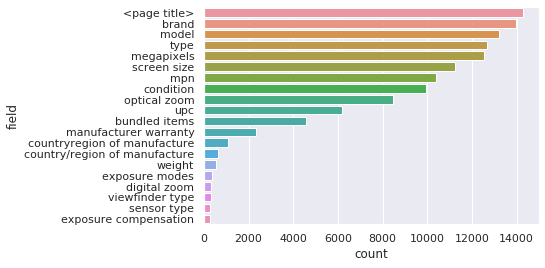
\includegraphics[width=0.9\columnwidth]{../figures/filled_fields.png}
\caption{Non-empty field count in specifications.}
\label{fig:filled_fields}
\end{figure} 

\textbf{Few labels}. Only around 300 thousand pairs were labeled of the 4.5 million total possible pairs. 

\subsection{Results}

With our best approach, described in this article we obtained an F1-score of \textbf{0.9}, which put us in top-20 on the contest leaderboard. This result was in-line with our cross-validation results.

\section{Discussion}

\subsection{Experiments with triplet loss and LSH}

Our initial attempt at reducing the number of pairs to compare was the following. First, produce a latent space embedding of specification page titles, such that specifications describing the same real-world product would appear close in that latent space, and others would be far. Then, build an index on these embeddings, so that retrieving the closest neighbors of a specification is fast. Finally, for each embedding, retrieve the closest neighbors, use the classifier model on the pairs $(embedding, neighbor)$. This would ensure that only similar specifications are evaluated.

We used a triplet loss neural network ~\cite{hoffer2015deep} to produce the embeddings and Annoy locally sensitive hashing~\cite{annoy} library to build the index.

However, recall achieved by this model was close to zero. Embeddings produced for the labeled instances were decently separated in latent space, but the model performed poorly on previously unseen data, as seen in Figure~\ref{fig:pairwise_dists}. 

\begin{figure}
\centering
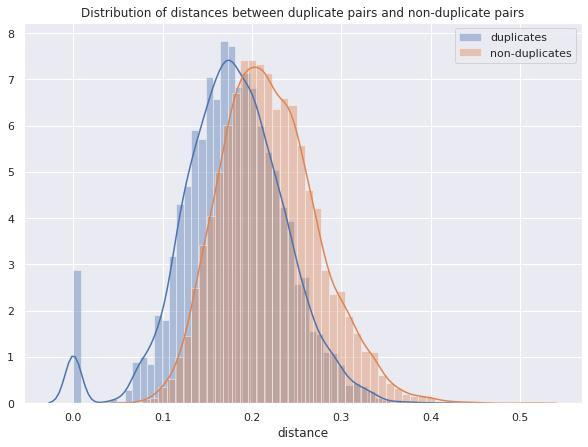
\includegraphics[width=0.9\columnwidth]{../figures/pairwise_dists.jpg}
\caption{Distributions of distances between pairs describing the same camera (duplicates) and pairs describing different cameras (non-duplicates)}
\label{fig:pairwise_dists}
\end{figure} 

Our hypothesis is that the labeled dataset did not contain enough information to produce a decent embedding for the whole dataset.

\subsection{Experiments with graph-based features}

At its core "describes the same camera model" is a transitive relationship on camera specifications. We thought hard about a way to provide information about transitivity to our classifier. One hypothesis was to use graph-based features. First, make a graph based on some distance metric between specification page titles. Let each specification be a vertex of the graph. If the distance between two specifications is below some threshold, produce an edge between their corresponding vertices. Then pairwise features like the number of common neighbors could be computed for each pair of specifications.

We attempted to create such a graph based on Levenstein ratio with a threshold of $0.9$. For reasons unknown to us, the features obtained from this graph did not provide any improvement to our model.

\section{Conclusions}

This project was a challenging task. It required us to build a model that is both fast and performant. Using preprocessing techniques, a way to reduce the subset of compared pairs to specifications of the same brand and an ensemble of classifiers we managed to achieve a decent result. Our best solution was ranked among the top 20 in the contest.


\bibliographystyle{ACM-Reference-Format}
\bibliography{sample-bibliography}

\end{document}
